\subsection{Dyna-Q in Modern Notation}
\label{section:fc_dyna_q}

The previous section traced two parallel origins of model-based reinforcement learning in 1990, one from the dynamic-programming tradition and one from the recurrent-neural-network tradition. This section develops the canonical instantiation of Sutton's side of that origin story, the Dyna-Q algorithm, in proper notation. Dyna-Q combines tabular $Q$-learning with a one-step deterministic model of the environment and applies $K$ planning updates per real interaction step. It is the template that the deep-learning era inherits and modifies, and it is the reference point that the algorithms chapter (\S\ref{section:rl_algorithms}) points to whenever model-based methods enter the discussion. The section gives the algorithm in formal notation, states the empirical headline from Sutton's original gridworld experiment, and then isolates the two architectural commitments that survive every subsequent reformulation of the idea.

\subsubsection{Algorithm}
\label{section:fc_dyna_q_algorithm}

Fix a finite Markov decision process with state space $\mathcal{S}$ and action space $\mathcal{A}$. Let $Q : \mathcal{S} \times \mathcal{A} \to \mathbb{R}$ denote the tabular action-value function the agent maintains over the course of interaction. Let $\widehat P(s' \mid s, a)$ denote the learned transition model and $\widehat r(s, a)$ the learned reward model; together these form the agent's internal forecaster of its environment. The remaining objects are a step size $\alpha \in (0, 1]$, a discount factor $\gamma \in [0, 1)$, an exploration parameter $\varepsilon \in (0, 1)$, and a planning horizon $K \in \mathbb{N}$ counting the number of synthetic updates applied per real step. The agent initializes $Q$, $\widehat P$, and $\widehat r$ to arbitrary values and then proceeds as follows.

For each step $t$:
\begin{enumerate}
  \item Observe the current state $s$ and select an action $a \in \arg\max_{a'} Q(s, a')$ with $\varepsilon$-greedy exploration, breaking ties uniformly at random.
  \item Execute $a$ in the environment and observe the reward $r$ and the next state $s'$.
  \item Direct RL update,
        \[ Q(s, a) \leftarrow Q(s, a) + \alpha \big[ r + \gamma \max_{a''} Q(s', a'') - Q(s, a) \big]. \]
  \item Model update, $\widehat r(s, a) \leftarrow r$ and $\widehat P(\cdot \mid s, a) \leftarrow \delta_{s'}$, recording the most recent observed transition as a deterministic prediction.
  \item Planning. Repeat $K$ times, on each iteration sampling a previously-visited pair $(\tilde s, \tilde a)$ uniformly from the agent's experience, querying $\widehat r(\tilde s, \tilde a)$ and $\widehat P(\cdot \mid \tilde s, \tilde a)$ to obtain a synthetic transition $(\tilde r, \tilde s')$, and applying the same $Q$-update as in step 3,
        \[ Q(\tilde s, \tilde a) \leftarrow Q(\tilde s, \tilde a) + \alpha \big[ \tilde r + \gamma \max_{a''} Q(\tilde s', a'') - Q(\tilde s, \tilde a) \big]. \]
\end{enumerate}

Step 3 is the tabular $Q$-learning update of \citet{WatkinsDayan1992}, who prove that under decreasing step sizes satisfying $\sum_t \alpha_t = \infty$ and $\sum_t \alpha_t^2 < \infty$ and infinite visitation of every state-action pair, $Q$ converges with probability one to the optimal action-value $Q^\star$, the fixed point of the Bellman optimality operator $\mathcal{T}^\star$ defined by $(\mathcal{T}^\star Q)(s, a) = \mathbb{E}_{s' \sim P^\star(\cdot \mid s, a)}[r(s, a) + \gamma \max_{a'} Q(s', a')]$. The operator is a $\gamma$-contraction in the sup norm, which is the technical ingredient that powers the proof. Step 5 applies the same update with $P^\star$ and $r$ replaced by the learned $\widehat P$ and $\widehat r$; convergence of the full planning-and-learning loop has no closed-form guarantee in the tabular case beyond the consistency of $\widehat P$ and $\widehat r$ under the agent's visitation distribution, and the function-approximation setting is studied via Lipschitz-on-model arguments (\citealt{Asadi2018Lipschitz}, discussed in \S\ref{section:fc_synthesis_fails}) rather than by a single contraction.

The conceptual content of the indirect-versus-direct distinction collapses into a single observation. Steps 3 and 5 apply identical update rules to identical-looking $(s, a, r, s')$ tuples. The only difference is the provenance of the tuple. In step 3 the tuple is sampled from the true transition kernel of the environment by acting; in step 5 the tuple is sampled from the agent's learned model. Planning, in this architecture, is not a separate algorithm with its own update rule. It is the same update rule applied to model-generated rather than environment-generated experience, and the ratio $K$ is the single lever that controls how heavily the agent leans on its model relative to fresh interaction.

\subsubsection{Empirical headline}
\label{section:fc_dyna_q_empirics}

\citet{sutton1990} reports a gridworld maze experiment that fixes the empirical claim. The agent navigates a tabular maze with deterministic transitions and sparse reward, learning under three settings of the planning horizon, $K \in \{0, 5, 50\}$. Setting $K = 0$ recovers plain $Q$-learning, since the planning loop is skipped and only the direct RL update of step 3 fires per interaction. With $K = 50$, the agent reaches near-optimal performance in roughly three episodes; with $K = 0$, the same level of performance requires roughly twenty-five episodes. The ratio of episodes is the original planning-amplification claim. Each real step in the $K = 50$ variant carries the policy-improvement value of about fifty steps in the $K = 0$ variant, at the cost of additional internal computation and a learned model that must be accurate enough for the synthetic updates to be informative. A blocking-maze variant in the same paper shows that a small exploration bonus permits the agent to recover after the environment changes, addressing the obvious failure mode that comes with relying on a learned model.

\subsubsection{Two architectural commitments}
\label{section:fc_dyna_q_architecture}

The first commitment is that the model class is left unspecified. The algorithm box above uses a deterministic one-step Dirac model $\widehat P(\cdot \mid s, a) \leftarrow \delta_{s'}$, but this choice is incidental to the architecture. Sutton describes the model as ``probabilistic and oftentimes incorrect,'' which is the conceptual move that allows every subsequent paper to plug a different model class into the same outer loop without changing anything else. The deep era exercises this openness across diverse model classes. \citet{HaSchmidhuber2018} use a convolutional variational autoencoder paired with a mixture-density recurrent network, treated in \S\ref{section:fc_ha_schmidhuber}. The Recurrent State-Space Model that powers the PlaNet and Dreamer lines, treated in \S\ref{section:fc_rssm}, couples a deterministic recurrent path with a stochastic latent. MuZero, the value-aware end of the spectrum treated in \S\ref{section:fc_value_aware}, dispenses with observation reconstruction entirely and trains the model only against quantities that enter the planner's value calculation. The MBPO line, treated in \S\ref{section:fc_mbpo}, uses a deep ensemble of probabilistic feed-forward networks. The outer loop in each of these is recognizably Dyna; the model class is the variable that distinguishes them.

The second commitment is that the inner loop applies the same Bellman update on simulated and real data. Step 5 of the algorithm is not a distinct planning operator; it is step 3 with a different source of transitions. This single fact is what permits Dyna to unify direct and indirect reinforcement learning into one architecture rather than two competing approaches. In the dynamic-programming tradition before Sutton, indirect methods estimated a model and then ran value iteration on it as a separate batch computation, while direct methods updated values from interaction without any model. Dyna eliminates the wall between these two camps by routing both kinds of transitions through the same temporal-difference update. The architectural consequence is that the agent does not need to choose between learning from interaction and learning from a model; it can do both, and the ratio $K$ tunes the mixture. Every subsequent model-based method in this chapter inherits this commitment, whether it uses tabular updates, fitted $Q$-iteration, soft actor-critic, or an MPC controller as its inner loop. Read in economics terms, Dyna is adaptive learning with simulated experience added between observations. The sample-efficiency claim that follows is not a free lunch; simulated experience is useful only where the learned model is accurate enough for the planner's purpose, and most of the failure modes the chapter encounters later are forms of that purpose-relative inaccuracy.

\subsubsection{Simulation Study: Planning Amplification in the Blocking Maze}
\label{section:fc_dyna_q_sim}

This study is the chapter's first empirical study and is designed to make three claims quantitative. The first is the planning-amplification claim of \citet{sutton1990}: that on the same maze and the same environment-step budget, the value of each real interaction grows roughly in proportion to the number of model-based planning updates applied between interactions. The second is the diagnosis of why plain $\varepsilon$-greedy $Q$-learning is too slow on a sparse-reward tabular problem of this size and discount, an observation the literature often takes as given without quantification. The third is the model-staleness failure mode that comes with relying on a learned model; the experiment flips the wall mid-experiment to expose whether agents that trust their old model can recover. Figure~\ref{figure:fc_dyna_maze_layout} renders the two phases of the environment side by side.

\begin{figure}[ht]
  \centering
  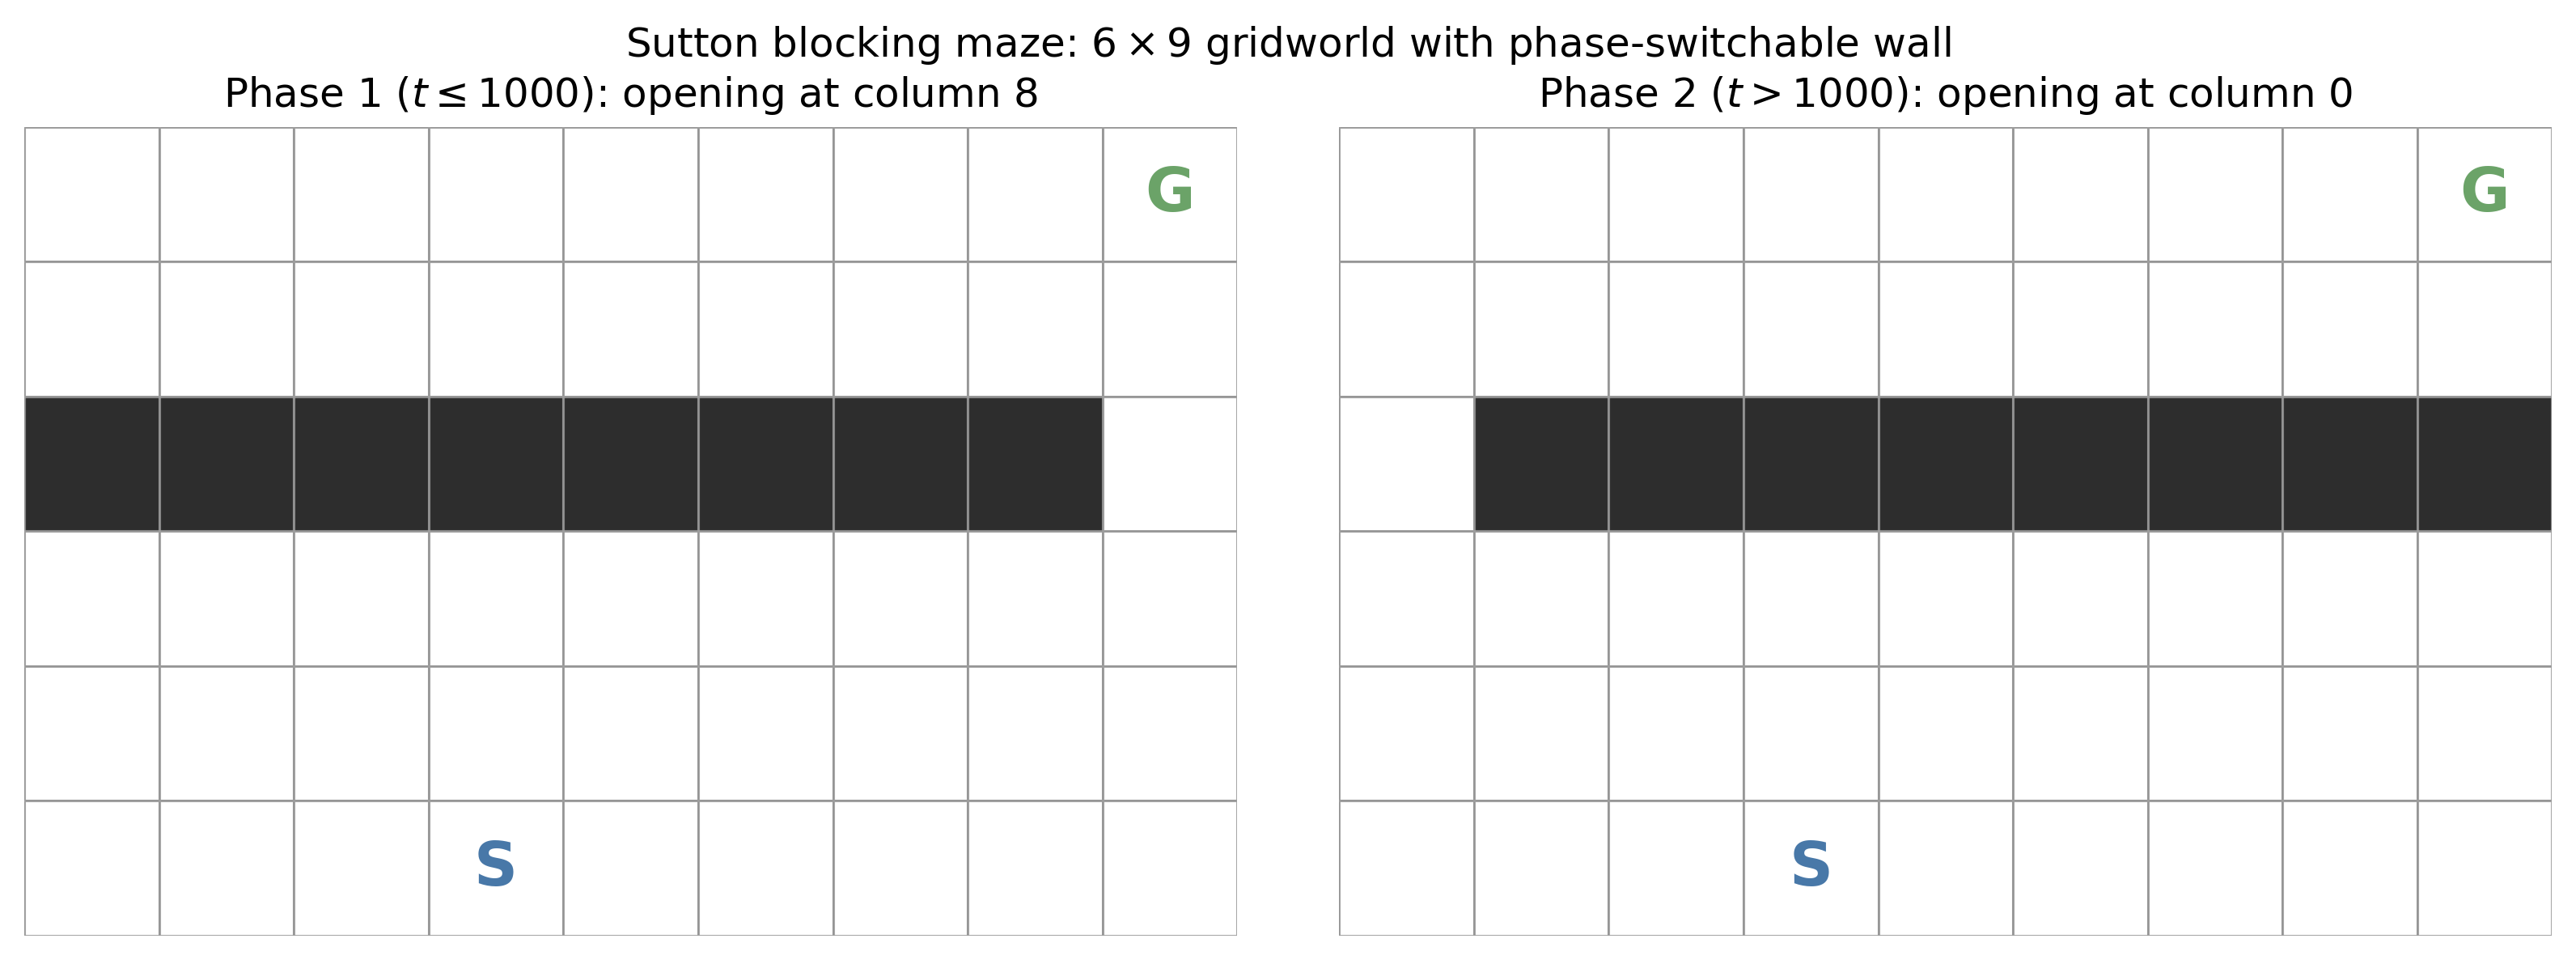
\includegraphics[width=0.95\textwidth]{../ch12_world_models/sims/dyna_maze_layout.png}
  \caption{Sutton blocking maze. The agent starts at $S$ and aims for the goal at $G$; the only opening in the wall along row two shifts from column eight in Phase 1 to column zero in Phase 2 at environment step $t = 1000$. The flip is not signaled to the agent and triggers the model-staleness failure mode that the experiment is designed to expose.}
  \label{figure:fc_dyna_maze_layout}
\end{figure}

\paragraph*{Why plain $Q$-learning is slow on this maze.}%
The diagnosis is quantitative. With $\gamma = 0.95$, $\alpha = 0.1$, $\varepsilon = 0.1$, $Q$-values initialized to zero, and a reward signal that is identically zero everywhere except at the goal, the agent reaches its first goal essentially by random walk; the expected hitting time of a single random walker from $S$ to $G$ on the open part of this $6 \times 9$ grid is several hundred steps. Each goal-reach updates exactly one entry of $Q$ by $\alpha \cdot 1 = 0.1$ toward the optimal value $\gamma^{d - 1}$, where $d$ is the path length from the parent state. Propagating that signal back to the start state requires a chain of subsequent goal-reaches at the right places, and $\varepsilon$-greedy noise at $\varepsilon = 0.1$ diverts the agent off its currently-best path on one in ten steps. The chance of stringing together a long enough sequence of goal-reaches to back the value all the way to $S$ within a few hundred environment steps is correspondingly small. This is the precise form of the slow-per-step-propagation claim that Dyna-Q is designed to address by replaying each successful real transition $K$ times against the model between every pair of real steps.

\paragraph*{Setup.}%
The environment is the $6 \times 9$ deterministic gridworld of \citet{sutton2018}, with start at row five column three and goal at row zero column eight. Actions are the four cardinal moves; transitions are deterministic; the reward is one on goal arrival and zero elsewhere; the discount factor is $\gamma = 0.95$. The wall along row two has its only opening at column eight during Phase 1 ($t \le N_1$ with $N_1 = 1000$) and at column zero during Phase 2 ($N_1 < t \le N_1 + N_2$ with $N_2 = 2000$). The phase flip happens automatically at $t = N_1$ and is not signaled. The total interaction budget is $N_1 + N_2 = 3000$ environment steps, the per-episode step cap is two hundred, and the experiment runs over thirty independent seeds with $\alpha = 0.1$, $\varepsilon = 0.1$, and zero-initialized $Q$.

\paragraph*{Models.}%
Five agents share the budget. Plain $Q$-learning with $K = 0$ is the direct-RL baseline, applying only the temporal-difference update of \citet{WatkinsDayan1992} per real step. Dyna-Q with $K = 5$ applies five model-based replays per real step from a tabular Dirac model, and Dyna-Q with $K = 50$ applies fifty; both implement the algorithm box of \S\ref{section:fc_dyna_q_algorithm} with the planning-step count set to the named value. Dyna-Q+ with $K = 50$ adds the exploration bonus $\kappa \sqrt{\tau(s, a)}$ to planning targets, with $\tau(s, a)$ the time since the state-action was last visited and $\kappa = 10^{-4}$, instantiating the primitive curiosity mechanism that connects to the prediction-error and ensemble-disagreement variants of \S\ref{section:fc_synthesis_fails}. The fifth agent applies REINFORCE on imagined rollouts under a learned forward model, related to the Schmidhuber 1990 controller-model architecture of \S\ref{section:fc_origins_schmidhuber} but distinct in the gradient pathway, since the original 1990 formulation propagates analytic gradients through a differentiable model into the controller while the variant used here treats the rollout as a stochastic-policy estimator. The agent uses two small multilayer perceptrons: a model network $M_\theta$ mapping one-hot state plus one-hot action to next-state logits, fit on observed transitions by cross-entropy, and a controller network $C_\phi$ mapping one-hot state to action logits, fit by a REINFORCE policy-gradient estimator on imagined trajectories rolled forward through $M_\theta$. Both networks have a single thirty-two-unit hidden layer; planning calls happen every ten real steps with sixteen imagined trajectories of length ten and a moving-average baseline. This is the third 1990-era treatment of the same loop, sitting alongside Sutton's tabular Dyna and the two Dyna-Q variants of $K \in \{5, 50\}$.

\paragraph*{Results.}%
Figure~\ref{figure:fc_dyna_maze} and Table~\ref{table:fc_dyna_maze} report cumulative environment reward across the thirty seeds with mean and standard error bands, with rows in rank order by total reward at $t = 3000$. Dyna-Q at $K = 50$ leads with $52.0 \pm 4.2$ total goal-reaches, Dyna-Q+ at $K = 50$ follows at $47.0 \pm 4.4$, Dyna-Q at $K = 5$ at $39.2 \pm 4.7$, the Schmidhuber controller-model agent at $4.0 \pm 0.4$, and plain $Q$-learning closes the field at $3.5 \pm 0.5$. The top of the table reproduces the planning-amplification claim of \citet{sutton1990} cleanly under this budget; each real interaction in the $K = 50$ run carries roughly an order of magnitude more policy-improvement weight than the same interaction in $K = 0$, because the synthetic updates of Step 5 propagate the learned reward back through the state graph between every pair of real steps. Dyna-Q+ at $K = 50$ pays a small Phase 1 cost of about five reward units relative to plain Dyna-Q because the exploration bonus eats slightly into exploitation. The cost remains modest because the implementation follows \citet{sutton2018} §8.3 and registers all four actions at every visited state with $\tau = 0$ on first encounter, so the bonus drives discovery of untried actions rather than only perturbing the values of already-tried ones. The Schmidhuber agent tracks plain $Q$-learning on this maze rather than tabular Dyna-Q because the gradient-based fit of the neural model needs many real samples to specialize from a random initialization, and at three thousand environment steps it has not yet accumulated enough buffer entries near the goal for the REINFORCE estimator to drive the controller toward the discovered path. Phase 2 reveals the recovery story. Dyna-Q at $K = 50$ continues to gain reward at the rate of $9.8 \pm 4.0$ over the remaining two thousand steps because $\varepsilon$-greedy noise eventually exposes the new corridor and the planning loop quickly retrains the model. Dyna-Q+ matches that rate at $9.6 \pm 2.8$, with the curiosity bonus driving the agent to revisit untried actions on the opposite side of the wall. The two rates are statistically indistinguishable on a Welch $t$-test with $p > 0.5$, and the Phase 1 deficit shrinks but does not close by $t = 3000$. \citet{sutton2018} Figure 8.5 reports Dyna-Q+ recovering faster than Dyna-Q after the maze flip; the thirty-seed reproduction here does not separate the two methods on the recovery slope, and a longer post-flip budget or a larger bonus coefficient than $\kappa = 10^{-4}$ would likely be needed to recover the Fig.~8.5 effect size cleanly. The Schmidhuber agent's Phase 2 gain of $1.5 \pm 0.2$ is only modestly above plain $Q$-learning's $0.6 \pm 0.2$ and tracks the same slow trajectory. The verdict is that the planning-amplification claim of \citet{sutton1990} reproduces cleanly under this budget, with tabular Dyna-Q at $K = 50$ delivering an order-of-magnitude improvement over $K = 0$, and Dyna-Q+ with faithful untried-action initialization recovering at the same Phase 2 rate as plain Dyna-Q while paying only a small Phase 1 exploration cost. The neural controller-model agent pays the cost of fitting a learned model from scratch on a tabular task that does not need a neural model to represent. The three 1990-era commitments, the deterministic Dirac model with $K$ planning steps, the exploration bonus as a stale-model fix, and a learned neural model with rollout-based policy gradients, sit at three different points on the empirical frontier, with tabular Dyna-Q dominating at this scale and the neural-model architecture's promise visible only when the state space is large enough that tabular methods cannot follow.

\begin{figure}[ht]
  \centering
  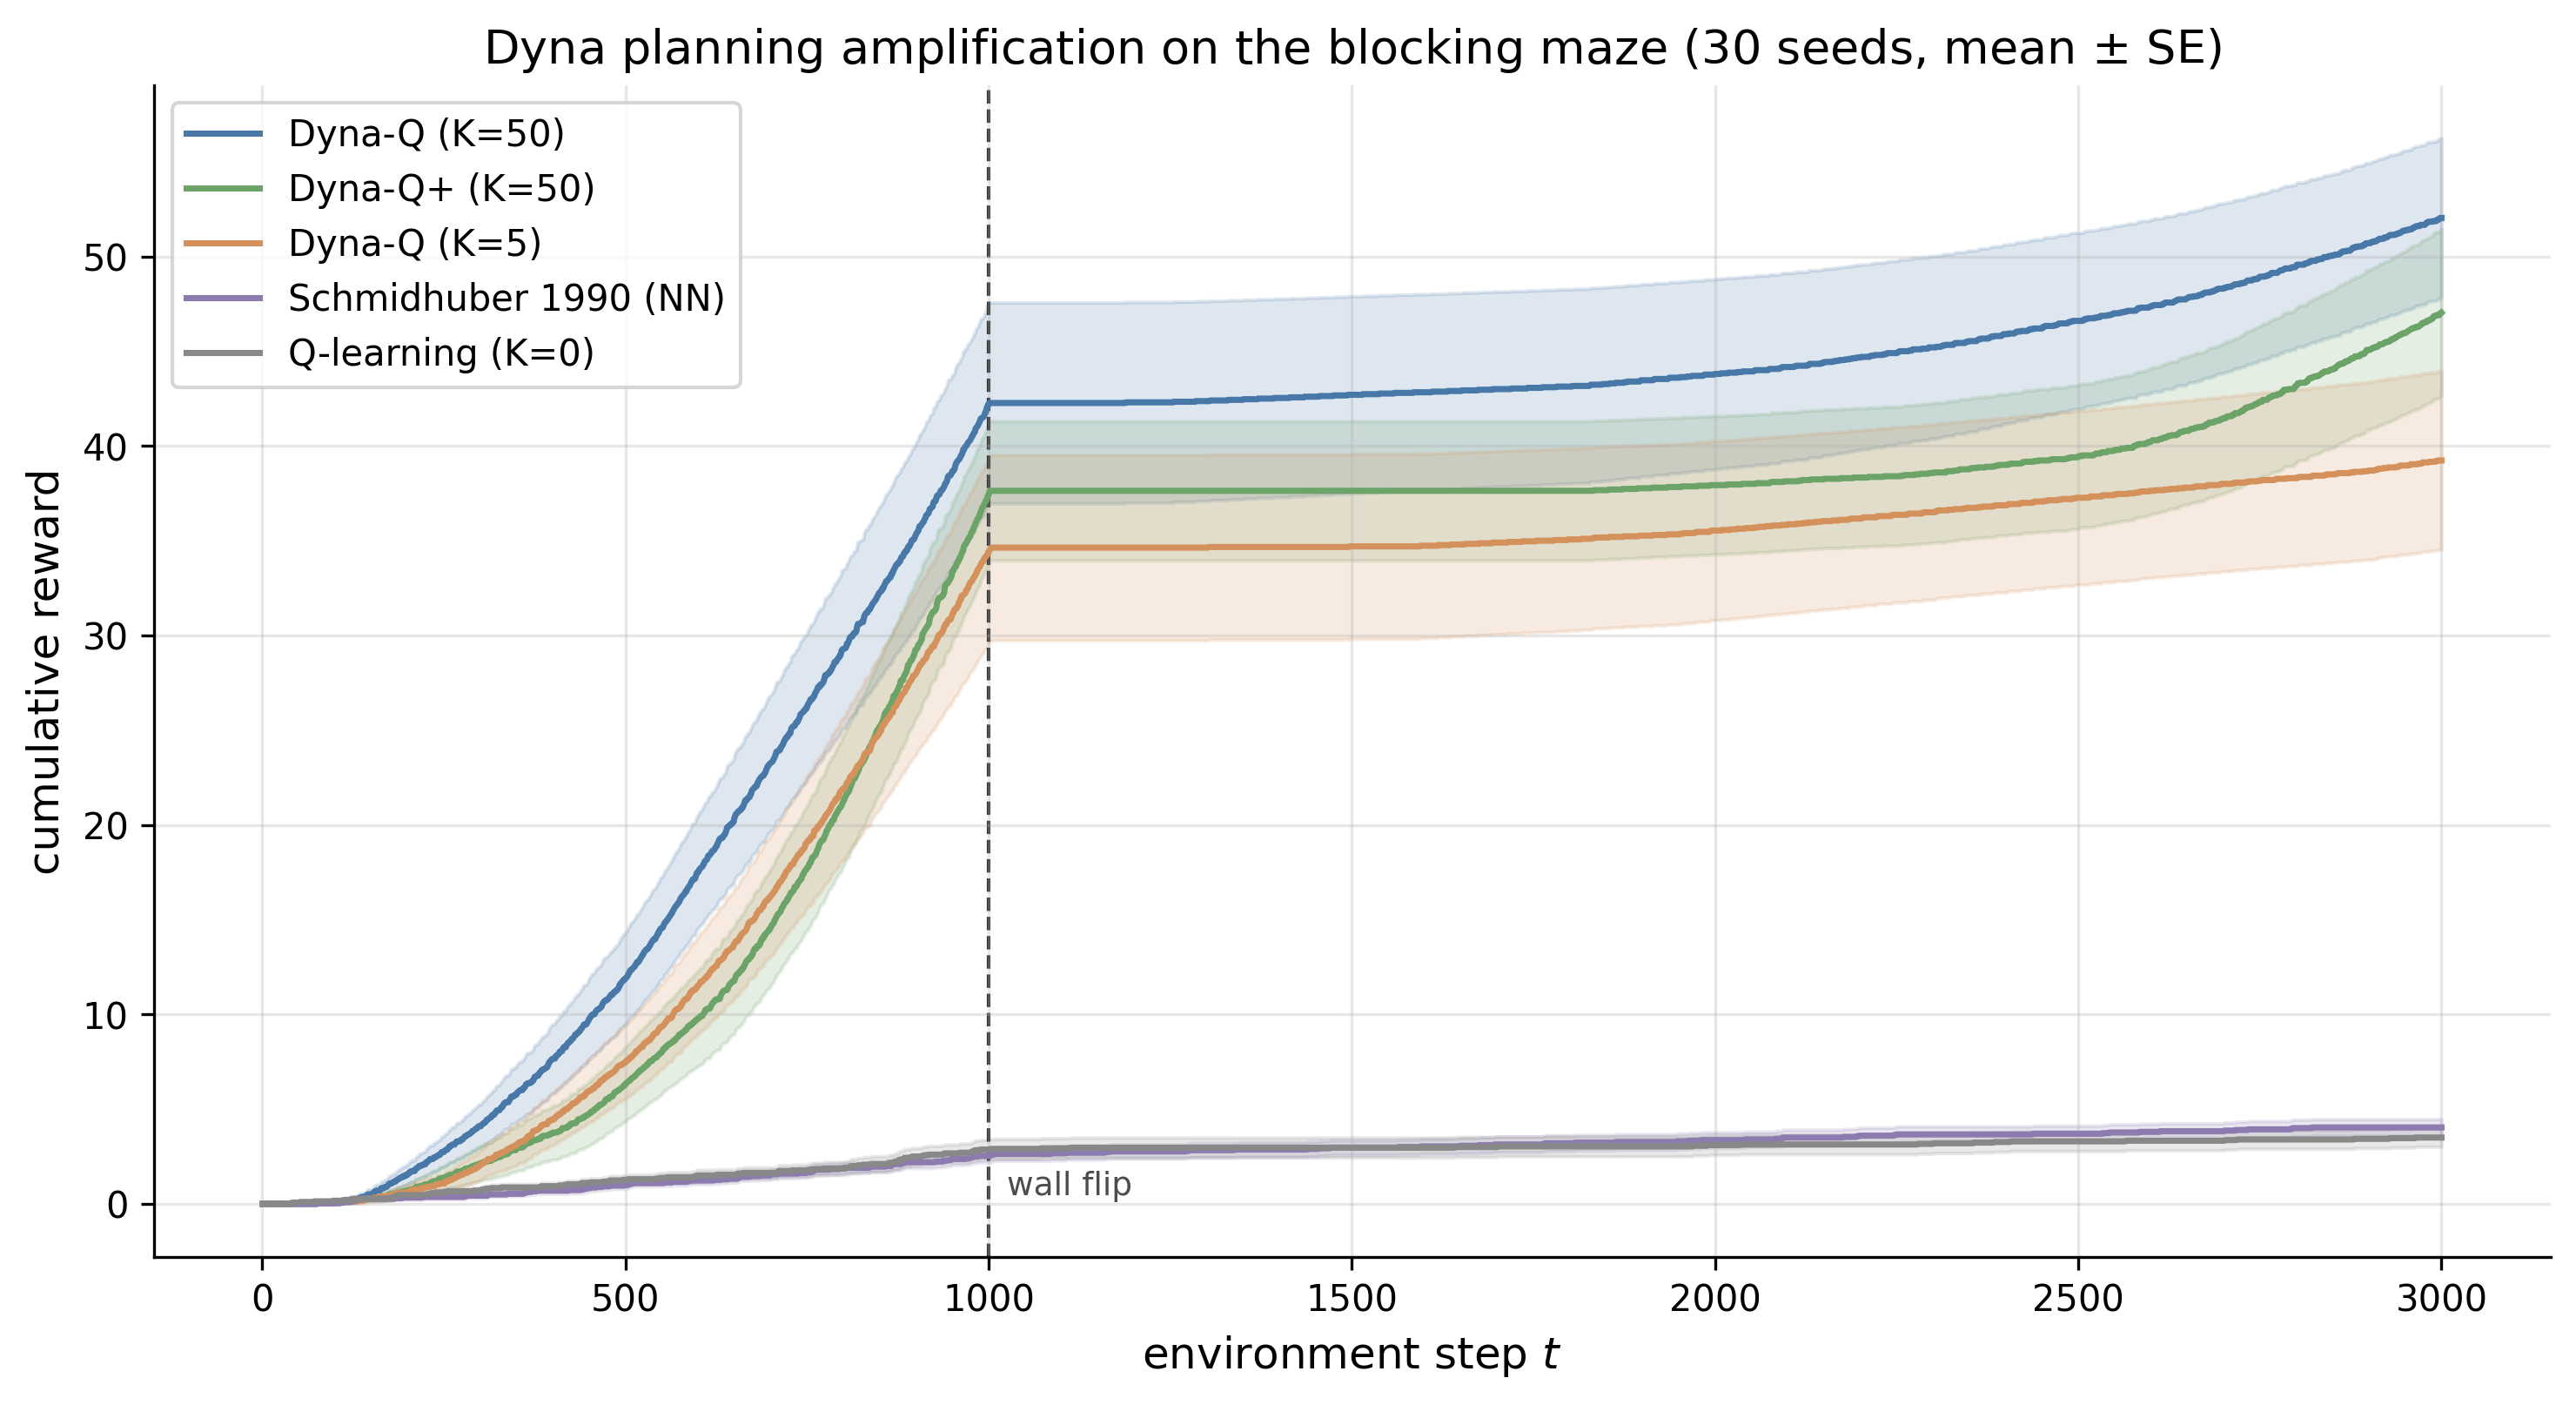
\includegraphics[width=0.95\textwidth]{../ch12_world_models/sims/dyna_maze.png}
  \caption{Cumulative reward on the blocking maze for five agents under a shared three-thousand-step environment budget. The dashed vertical line marks the wall flip at $t = 1000$. Lines are means and shaded bands are one standard error across thirty seeds.}
  \label{figure:fc_dyna_maze}
\end{figure}

\begin{table}[ht]
  \centering
  \caption{Cumulative reward on the blocking maze. End of Phase 1 is at $t = 1000$; Phase 2 gain is the increase over the remaining two thousand steps; Total is the value at $t = 3000$. Mean $\pm$ standard error across thirty seeds.}
  \label{table:fc_dyna_maze}
  % Cumulative reward at end of Phase 1 (t=1000), gain over Phase 2 (last 2000 steps), and total at t=3000.
% Mean +/- SE across 30 seeds.
\begin{tabular}{lrrr}
\toprule
Agent & End of Phase 1 & Phase 2 gain & Total ($t = 3000$) \\
\midrule
Dyna-Q (K=50) & 42.2 $\pm$ 5.3 & 9.8 $\pm$ 4.0 & 52.0 $\pm$ 4.2 \\
Dyna-Q+ (K=50) & 37.4 $\pm$ 3.7 & 9.6 $\pm$ 2.8 & 47.0 $\pm$ 4.4 \\
Dyna-Q (K=5) & 34.4 $\pm$ 4.9 & 4.8 $\pm$ 3.0 & 39.2 $\pm$ 4.7 \\
Schmidhuber 1990 (NN) & 2.5 $\pm$ 0.3 & 1.5 $\pm$ 0.2 & 4.0 $\pm$ 0.4 \\
Q-learning (K=0) & 2.9 $\pm$ 0.5 & 0.6 $\pm$ 0.2 & 3.5 $\pm$ 0.5 \\
\bottomrule
\end{tabular}

\end{table}
